\documentclass{ctexart}
\usepackage{multicol}
\usepackage{amsmath, amsfonts, amssymb}
\usepackage{tikz, tkz-graph}
\usepackage{geometry}
\special{dvipdfmx:config z 0} % delete this when release

\usetikzlibrary{positioning}

\geometry{a4paper,scale=0.8}

\title{集合论与图论~作业10-11}
\author{庄嘉毅}
\date{October 2022}

\def\QED{\hfill $\square$}
\def\st{\textrm{s.t.}\,}
\def\pair#1{\left\langle #1 \right\rangle}
\def\conj{\mathrel{\wedge}}
\def\disj{\mathrel{\vee}}
\def\equ{\mathrel{\Leftrightarrow}}
\def\restr{\mathbin{\upharpoonright}}
\def\ple{\mathrel{\preccurlyeq}}
\DeclareMathOperator{\dom}{dom}
\DeclareMathOperator{\ran}{ran}
\DeclareMathOperator{\fld}{fld}
\DeclareMathOperator{\card}{card}
\DeclareMathOperator{\e}{e}

\everymath{\displaystyle}
% \linespread{2}

\begin{document}

\maketitle

\section*{习题七}

\paragraph*{1} 设 $G$ 有 $n$ 个顶点, 由握手定理,
$2\times 16\le 3\times 4+4\times 3 + 2(n-3-4)=2n+10$,
解得 $n\ge 11$.

\begin{figure}[ht]
    \centering
    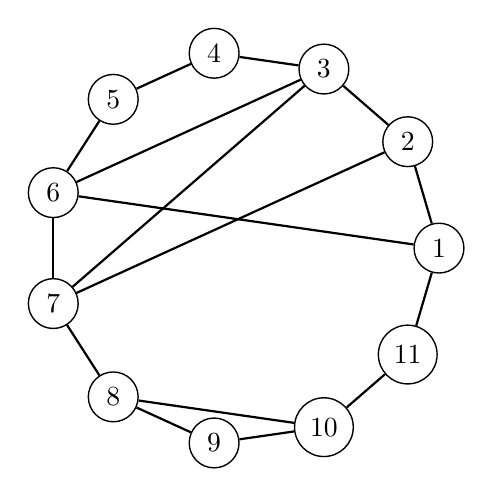
\begin{tikzpicture}
        \GraphInit[vstyle=Normal]
        \Vertices[unit=2.5]{circle}{1,2,3,4,5,6,7,8,9,10,11}
        \Edges(1,2,3,4,5,6,7,8,9,10,11,1)
        \Edges(1,6,3)
        \Edges(2,7)
        \Edges(3,7)
        \Edges(10,8)
    \end{tikzpicture}
    \caption{第1题图}
    \label{fig:1}
\end{figure}

如图 \ref{fig:1} 所示,存在 11 个顶点的图满足条件,因此顶点数的最小值为11.

\paragraph*{2} 设 $G$ 有 $n$ 个5度顶点, $9-n$个6度顶点, 由握手定理,
$5n+6(9-n)\equiv 0\pmod 2$, 故 $2\mid n$, 因此 $n\ne 5$,
即 $n\ge 6$ 或 $n\le 4$ , 也即 $n\ge 6$ 或 $9-n\ge 5$. \QED


\paragraph*{3} 记多面体有 $f$个面,每个面的棱数分别为$e_1,e_2,\ldots,e_f$,
由握手定理,
\begin{gather*}
    \sum_{i=1}^f e_i \equiv 0 \pmod 2
\end{gather*}

若 $e_i$ 均为奇数, 那么
\begin{gather*}
    \sum_{i=1}^f e_i \equiv \sum_{i=1}^f 1 \equiv f \pmod 2
\end{gather*}

故此时 $f$ 只能为偶数. 因此不存在有奇数个面且每个面均有奇数条棱的多面体. \QED

\paragraph*{5} 由握手定理, $3n=2m$, 又 $2n-3=m$, 解得 $n=6,m=9$.

\begin{figure}[ht]
    \centering
    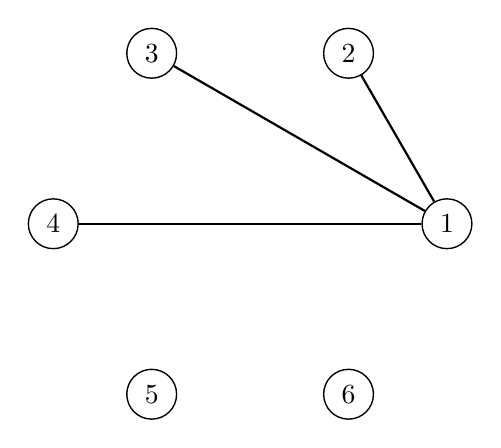
\begin{tikzpicture}
        \GraphInit[vstyle=Normal]
        \Vertices[unit=2.5]{circle}{1,2,3,4,5,6}
        \Edges(1,2)
        \Edges(1,3)
        \Edges(1,4)
    \end{tikzpicture}
    \caption{第5题图}
    \label{fig:5}
\end{figure}

% 教材习题7: 3,5,11,14,16,18,22,25
\end{document}
